\documentclass[tikz,border=5pt]{standalone}
\usepackage{tikz}
\usetikzlibrary{3d}
\usepackage{amssymb}
\usepackage{subfig}
\usepackage{float}
%\usepackage{subfigure}
\usepackage{hyperref}
\hypersetup{colorlinks=true,linkcolor=blue}
\usepackage{amsmath}
\usepackage{tikz}
\usepackage{lipsum}
\usetikzlibrary{arrows.meta}
\usetikzlibrary{arrows}
\usepackage{pstricks}
\usetikzlibrary{fadings}
%\usepackage{graphicx}
% \usepackage[nodots,nocompress]{numcompress}
\definecolor{ig}{rgb}{0.07, 0.53, 0.03}
\definecolor{cd}{rgb}{0.89, 0.0, 0.13}

\begin{document}
	
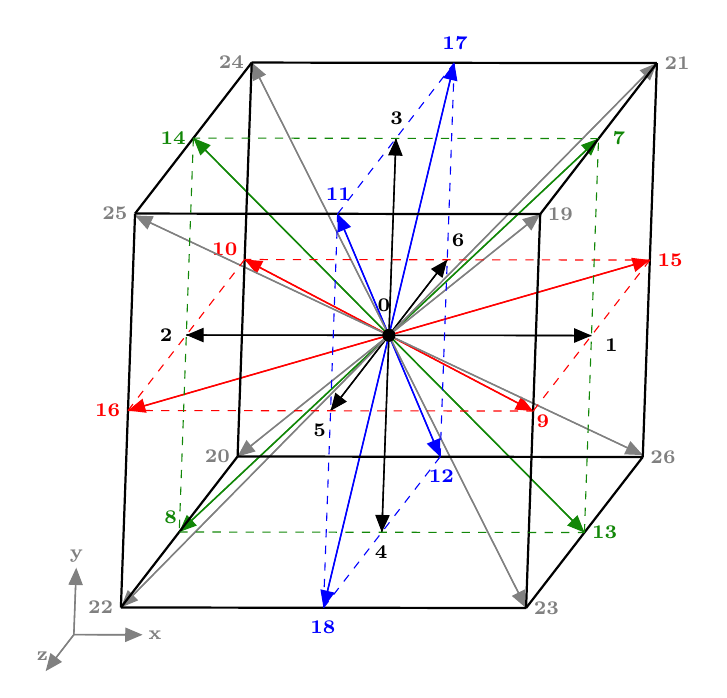
\begin{tikzpicture}[font=\scriptsize,scale=2.50,rotate around y=5,rotate around z=-2]
	\tikzset{
		myarrow/.style={
			draw=#1,
			fill=#1,
			solid,
			line width=0.2mm,
			preaction={-triangle 45,#1,thin,draw,shorten <=1mm, shorten >=0mm}
		}
	}


\draw[black,fill=black] (0,0,0)node[]{} circle(0.03cm); %node 0
 \draw (-0.03,0.15,0)node[]{$\mathbf{0}$};

% Node 1
%\draw[gray,fill=gray] (1,0,0)node[]{} circle(0.03cm);  %node 1
\path[myarrow=black, fill=red] (0,0,0) -- (1,0,0);
\draw (1.1,-0.05,0) node {$\mathbf{1}$};

% Node 2
%\draw[gray,fill=gray] (-1,0,0)node[]{} circle(0.03cm);  %node 2
\path[myarrow=black, fill=black] (0,0,0) -- (-1,0,0);
\draw (-1.1,0,0) node {$\mathbf{2}$};

% Node 3
%\draw[gray,fill=gray] (0,1,0)node[]{} circle(0.03cm);  %node 3
\path[myarrow=black, fill=black] (0,0,0) -- (0,1,0);
\draw (0,1.1,0) node {$\mathbf{3}$};

% Node 4
%\draw[gray,fill=gray] (0,-1,0)node[]{} circle(0.03cm);  %node 4
\path[myarrow=black, fill=black] (0,0,0) -- (0,-1,0);
\draw (0,-1.1,0) node {$\mathbf{4}$};

% Node 5
%\draw[gray,fill=gray] (0,0,1)node[]{} circle(0.03cm);  %node 5
\path[myarrow=black, fill=black] (0,0,0) -- (0,0,1);
\draw (-0.05,-0.1,1) node {$\mathbf{5}$};

% Node 6
%\draw[gray,fill=gray] (0,0,-1)node[]{} circle(0.03cm);  %node 6
\path[myarrow=black, fill=black] (0,0,0) -- (0,0,-1);
\draw (0.05,0.1,-1) node {$\mathbf{6}$};

% Node 7
%\draw[gray,fill=gray] (1,1,0)node[]{} circle(0.03cm);  %node 7
\path[myarrow=ig] (0,0,0) -- (1,1,0);
\draw (1.1,1,0) node[ig] {$\mathbf{7}$};

% Node 8
%\draw[gray,fill=gray] (-1,-1,0)node[]{} circle(0.03cm);  %node 8
\path[myarrow=ig] (0,0,0) -- (-1,-1,0);
\draw (-1.1,-1,-0.2) node[ig] {$\mathbf{8}$};

% Node 9
%\draw[gray,fill=gray] (1,0,1)node[]{} circle(0.03cm);  %node 9
\path[myarrow=red] (0,0,0) -- (1,0,1);
\draw (1.05,-0.05,1) node[red] {$\mathbf{9}$};

% Node 10
%\draw[gray,fill=gray] (-1,0,-1)node[]{} circle(0.03cm);  %node 10
\path[myarrow=red] (0,0,0) -- (-1,0,-1);
\draw (-1.1,0.05,-1) node[red] {$\mathbf{10}$};

% Node 11
%\draw[gray,fill=gray] (0,1,1)node[]{} circle(0.03cm);  %node 11
\path[myarrow=blue] (0,0,0) -- (0,1,1);
\draw (0,1.1,1) node[blue] {$\mathbf{11}$};

% Node 12
%\draw[gray,fill=gray] (0,-1,-1)node[]{} circle(0.03cm);  %node 12
\path[myarrow=blue] (0,0,0) -- (0,-1,-1);
\draw (0.01,-1.1,-1) node[blue] {$\mathbf{12}$};

% Node 13
%\draw[gray,fill=gray] (1,-1,0)node[]{} circle(0.03cm);  %node 13
\path[myarrow=ig] (0,0,0) -- (1,-1,0);
\draw (1.1,-1,0) node[ig] {$\mathbf{13}$};

% Node 14
%\draw[gray,fill=gray] (-1,1,0)node[]{} circle(0.03cm);  %node 14
\path[myarrow=ig] (0,0,0) -- (-1,1,0);
\draw (-1.1,1,0) node[ig] {$\mathbf{14}$};

% Node 15
%\draw[gray,fill=gray] (1,0,-1)node[]{} circle(0.03cm);  %node 15
\path[myarrow=red] (0,0,0) -- (1,0,-1);
\draw (1.1,0,-1) node[red] {$\mathbf{15}$};

% Node 16
%\draw[gray,fill=gray] (-1,0,1)node[]{} circle(0.03cm);  %node 16
\path[myarrow=red] (0,0,0) -- (-1,0,1);
\draw (-1.1,0,1) node[red] {$\mathbf{16}$};

% Node 17
%\draw[gray,fill=gray] (0,1,-1)node[]{} circle(0.03cm);  %node 17
\path[myarrow=blue] (0,0,0) -- (0,1,-1);
\draw (0,1.1,-1) node[blue] {$\mathbf{17}$};

% Node 18
%\draw[gray,fill=gray] (0,-1,1)node[]{} circle(0.03cm);  %node 18
\path[myarrow=blue] (0,0,0) -- (0,-1,1);
\draw (0,-1.1,1) node[blue] {$\mathbf{18}$};

% Node 19
%\draw[gray,fill=gray] (1,1,1)node[]{} circle(0.03cm);  %node 19
\path[myarrow=gray] (0,0,0) -- (1,1,1);
\draw (1.1,1,1) node[gray] {$\mathbf{19}$};

% Node 20
%\draw[gray,fill=gray] (-1,-1,-1)node[]{} circle(0.03cm);  %node 20
\path[myarrow=gray] (0,0,0) -- (-1,-1,-1);
\draw (-1.1,-1,-1) node[gray] {$\mathbf{20}$};

% Node 21
%\draw[gray,fill=gray] (1,1,-1)node[]{} circle(0.03cm);  %node 21
\path[myarrow=gray] (0,0,0) -- (1,1,-1);
\draw (1.1,1,-1) node[gray] {$\mathbf{21}$};

% Node 22
%\draw[gray,fill=gray] (-1,-1,1)node[]{} circle(0.03cm);  %node 22
\path[myarrow=gray] (0,0,0) -- (-1,-1,1);
\draw (-1.1,-1,1) node[gray] {$\mathbf{22}$};

% Node 23
%\draw[gray,fill=gray] (1,-1,1)node[]{} circle(0.03cm);  %node 23
\path[myarrow=gray] (0,0,0) -- (1,-1,1);
\draw (1.1,-1,1) node[gray] {$\mathbf{23}$};

% Node 24
%\draw[gray,fill=gray] (-1,1,-1)node[]{} circle(0.03cm);  %node 24
\path[myarrow=gray] (0,0,0) -- (-1,1,-1);
\draw (-1.1,1,-1) node[gray] {$\mathbf{24}$};

% Node 25
%\draw[gray,fill=gray] (-1,1,1)node[]{} circle(0.03cm);  %node 25
\path[myarrow=gray] (0,0,0) -- (-1,0.99,1);
\draw (-1.1,1,1) node[gray] {$\mathbf{25}$};

% Node 26
%\draw[gray,fill=gray] (1,-1,-1)node[]{} circle(0.03cm);  %node 26
\path[myarrow=gray] (0,0,0) -- (1,-0.99,-1);
\draw (1.1,-1,-1) node[gray] {$\mathbf{26}$};


%Front square
% \draw [fill=orange] (-1,-1,1) rectangle (1,-1,1);
\draw[solid,thick] (-1,-1,1) -- (1,-1,1);
\draw[solid,thick] (1,-1,1) -- (1,1,1);
\draw[solid,thick] (1,1,1) -- (-1,1,1);
\draw[solid,thick] (-1,1,1) -- (-1,-1,1);

%Back square
\draw[solid,thick] (-1,-1,-1) -- (1,-1,-1);
\draw[solid,thick] (1,-1,-1) -- (1,1,-1);
\draw[solid,thick] (1,1,-1) -- (-1,1,-1);
\draw[solid,thick] (-1,1,-1) -- (-1,-1,-1);

%Edges
\draw[solid,thick] (-1,-1,1) -- (-1,-1,-1); % bottem left
\draw[solid,thick] (1,-1,1) -- (1,-1,-1); % bottem right
\draw[solid,thick] (-1,1,-1) -- (-1,1,1);  % top left
\draw[solid,thick] (1,1,-1) -- (1,1,1);  % top right

%mid planes
%x=0 plane
\draw[blue,dashed, thin] (0,-1,1) -- (0,-1,-1);
\draw[blue,dashed, thin] (0,-1,-1) -- (0,1,-1);
\draw[blue,dashed, thin] (0,1,-1) -- (0,1,1);
\draw[blue,dashed, thin] (0,1,1) --(0,-1,1);
%y=0 planed
\draw[red,thin,dashed] (-1,0,1) -- (1,0,1);
\draw[red,thin,dashed] (1,0,1) -- (1,0,-1);
\draw[red,thin,dashed] (1,0,-1) --  (-1,0,-1);
\draw[red,thin,dashed] (-1,0,-1) -- (-1,0,1);
%z=0 plane
\draw[ig,thin,dashed] (-1,-1,0) -- (1,-1,0);
\draw[ig,thin,dashed] (1,-1,0) -- (1,1,0);
\draw[ig,thin,dashed] (1,1,0) -- (-1,1,0);
\draw[ig,thin,dashed] (-1,1,0) -- (-1,-1,0);

\path[draw=gray,solid,line width=0.2mm,preaction={-triangle 45,gray,thin,draw,shorten >=-1mm}](-1.2,-1.1,1.1) -- (-0.9,-1.1,1.1);	%node x
\draw (-0.8,-1.1,1.1)node[gray]{$\mathbf{x}$};
\path[draw=gray,solid,line width=0.2mm,preaction={-triangle 45,gray,thin,draw,shorten >=-1mm}](-1.2,-1.1,1.1) -- (-1.2,-0.8,1.1);	%node y
\draw (-1.2,-0.7,1.1)node[gray]{$\mathbf{y}$};
\path[draw=gray,solid,line width=0.2mm,preaction={-triangle 45,gray,thin,draw,shorten >=-1mm}](-1.2,-1.1,1.1) -- (-1.2,-1.1,1.5);	%node z
\draw (-1.2,-1,1.65)node[gray]{$\mathbf{z}$};

\draw[black,fill=black] (0,0,0)node[]{} circle(0.03cm); %node 0
\end{tikzpicture}

	
	
\end{document}
